\chapter{Analisis dan Rancangan Klasifikasi Teks Berbahasa Indonesia Menggunakan \textit{Multi-lingual Language Model}}

Bab ini berisi analisis dan rancangan berkaitan dengan studi literatur pada bab sebelumnya. Oleh karena itu, bab ini akan terdiri dari analisis permasalahan dan rancangan solusi.

\section{Analisis Permasalahan}

	\subsection{Analisis Permasalahan Analisis Sentimen}
	Pada penelitian ini, digunakan dataset yang sama dengan dataset \parencite{FarhanKhodra2017}. Dataset tersebut merupakan ulasan-ulasan dari situs TripAdvisor yang kemudian dilabeli positif untuk nilai 3-5 dan negatif untuk nilai 1-2. Setiap ulasan, yang terdiri dari satu sampai tiga kalimat, dapat memiliki frasa sentimen di awal, di tengah, dan di akhir dokumen. Berikut contoh ulasan yang berlabel negatif.

	“Kemaren sengaja coba makan di marugame udon karena istri suka banget sama udon. jadi pesan lah yang kuah kaldu ayam, dan anak saya minta gorengan kroket. saya kira kuahnya langsung dari pancinya harusnya panas, tapi ternyata cuman hangat, yah kecewa juga sih, gorengannya juga sama udah dingin” 

	Dapat dilihat dari paragraf di atas, kalimat awal pada paragraf tersebut tidak mengandung sentimen apapun. Frasa sentimen baru ditemui di akhir paragraf. Berikut contoh ulasan yang berlabel positif.

	“berlokasi di pusat jakarta.. sangat mudah mengakses ke berbagai tempat strategis dan keramaian. hotel sangat bersih, pelayanan ramah dan makanan sesuai lidah indonesia atau western. sangat direkomendasikan.”

	Dapat dilihat dari paragraf di atas, frasa sentimen positif sudah langsung diutarakan pada awal paragraf. Tetapi tidak semua ulasan memiliki satu sentimen saja. Berikut ini adalah salah satu contoh ulasan pada dataset yang mengandung frasa sentimen negatif dan positif disaat bersamaan. 

	“Kelihatan dari luar memang menarik tempatnya. Suasananya juga cozy. Saat makan siang juga ramai pengunjung. AC tidak berasa, jadi lumayan panas di dalam. Memesan nasi dengan irisan slice pork belly, nasinya tanpa bumbu apa- apa jadi kering banget, irisan pork belly nya dominan lemak dan minyak. Kita dapat 6 slice, tapi sesudah makan slice ke 3, rasanya tidak sanggup lagi karena merasa eneg dengan lemak pork belly nya.”

	Dapat dilihat dari paragraf di atas, tiga kalimat pertama menunjukkan opini positif sedangkan 3 kalimat terakhir menunjukkan opini negatif. Tetapi berdasarkan analisis keseluruhan, dapat dilihat bahwa ulasan tersebut bersentimen negatif.

	Penelitian terkait oleh \parencite{FarhanKhodra2017} dan \parencite{CrisdayantiPurwarianti2019} sudah mengekplorasi berbagai jenis representasi dokumen dan topologi untuk menyelesaikan analisis sentimen level dokumen pada data tersebut. Meski sudah mendapatkan hasil, penelitian terkait sebelumnya belum mengeksplorasi penggunaan \textit{language model} dalam bentuk apapun, terlebih lagi penggunaan \textit{transfer learning} lintas bahasa.

	Perkembangan dalam bidang teknik pemrosesan teks dewasa ini telah memunculkan berbagai jenis \textit{language model} dan teknik pembangunannya. Salah satunya adalah \textit{language model} lintas bahasa bernama XLM oleh \parencite{LampleConneau2019} yang dibangun tanpa menggunakan korpus paralel atau kamus kata antar bahasa. Hal ini memungkinkan kita menggunakan representasi antar bahasanya untuk melatih model analisis sentimen bahasa Indonesia dengan dataset bahasa lainnya.

	\subsection{Analisis Permasalahan Klasifikasi Teks Ujaran Kebencian \& Kasar}


% Data adalah inti dari pembangunan sistem analisis sentimen. Sedikitnya data yang sudah dianotasi pada bahasa Indonesia menyulitkan pengembangan sistem analisis sentimen yang lebih akurat. Di lain hal, bahasa asing seperti bahasa Inggris memiliki jauh lebih banyak data yang sudah dianotasi. Teknik yang dapat memanfaatkan data dari bahasa asing untuk membangun sistem pemrosesan teks di bahasa Indonesia diperlukan.

% Teknik pemrosesan teks memungkinkan pembangunan ruang embedding antar bahasa. Dengan memanfaatkan representasi teks antar bahasa, dimungkinkan melatih classifier pada suatu bahasa dan menggunakannya pada bahasa lain seperti pada \parencite{Artetxe_Schwenk_2019}.

% Tidak hanya itu, gap antar domain yang menjadi ulasan pun dapat diselesaikan dengan teknik augmentasi yang \parencite{Lai_Oguz_Yang_Stoyanov_2019} kembangkan. 

\section{Rancangan Solusi}
	Berdasarkan analisis permasalahan yang dijabarkan pada bab sebelumnya, kita dapat menggunakan \textit{language model} antar bahasa XLM yang sudah dilatih dengan data dari 100 bahasa untuk memperkaya data analisis sentimen bahasa Indonesia. Diantara 100 bahasa yang sudah dilatih pada \textit{language model} XLM adalah bahasa Indonesia dan bahasa Inggris. Sub-bab selanjutnya akan membahas pemilihan dataset bahasa Inggris yang akan digunakan dan rancangan eksperimen untuk membuktikan tujuan dari tugas akhir ini.

	\subsection{Komponen Dataset Sumber Analisis Sentimen}
	Pada tugas akhir ini, dipilih dataset \textit{Yelp review}\footnote{\url{https://www.yelp.com/dataset/challenge}} dikarenakan jumlahnya dan kesesuaian domainnya dengan dataset TripAdvisor. Dataset polaritas Yelp reviews  dibangun dengan mengubah semua rating bintang 1 dan 2 menjadi negatif, dan rating bintang 3 dan 4 menjadi positif. Rincian dari dataset dapat dilihat pada tabel \ref{tab:detail_yelp_review}.

	\begin{table}[ht]
	    \centering
	    \caption{Rincian banyak data pada tiap partisi dan label di dataset \textit{Yelp review}.}
	    \begin{tabular}{@{}cc|cc@{}}
	    \multicolumn{1}{c}{} &\multicolumn{1}{c}{} &\multicolumn{2}{c}{Partisi} \\ 
	    \multicolumn{1}{c}{} & 
	    \multicolumn{1}{c|}{} & 
	    \multicolumn{1}{c}{\textit{Train}} & 
	    \multicolumn{1}{c}{\textit{Test}} \\ 
	    \cline{2-4}
	    \multirow[c]{2}{*}{\rotatebox[origin=tr]{90}{Label}}
	    & Positif  & 280.000 & 19.000   \\[1.5ex]
	    & Negatif  & 280.000 & 19.000   \\ 
	    \cline{2-4}
	    \end{tabular}
	    \label{tab:detail_yelp_review}
	\end{table}

	Sesuainya domain antara dataset sumber dan target sangat penting dikarenakan perbedaan domain dapat menurunkan performa klasifikasi \parencite{Lai_Oguz_Yang_Stoyanov_2019}. Hal ini dikarenakan sentimen tidak diutarakan dengan cara yang sama pada domain yang berbeda. Ulasan pada domain produk di toko \textit{e-commerce} akan berbeda dengan ulasan pada domain restoran. Pada domain produk di toko \textit{e-commerce}, ulasan akan berkutat pada aspek seperti kecepatan pengiriman barang, keselamatan barang, dan kualitas dari barang yang dibeli. Sedangkan ulasan pada domain restoran akan berkutat pada keramahan pelayanan, suasana restoran, dan kualitas makanan.

	\subsection{Komponen Dataset Bahasa Inggris Analisis Sentimen}
	
	\subsection{Komponen Dataset Bahasa Inggris Klasifikasi Ujaran Kebencian \& Kasar}

	\subsection{Komponen Klasifikasi}
	Skema eksperimen akan mengikuti eksperimen yang dilakukan oleh \parencite{LampleConneau2019} pada masalah klasifikasi antar bahasa dengan dataset XNLI \parencite{Conneau_Rinott_Lample_Williams_Bowman_Schwenk_Stoyanov_2018}. Pada eksperimennya, model yang sudah dilatih dengan data Wikipedia 100 bahasa ini di-\textit{finetune} dengan dataset tolak ukur klasifikasi. Lebih tepatnya, ditambahkan \textit{classifier} linier di atas \textit{hidden state}pertama dari \textit{language model} yang sudah di-\textit{pretrained}, yang kemudian semua parameternya dilatih pada dataset pelatihan NLI bahasa Inggris. Skema yang sama akan digunakan dengan sumber bahasa Inggris dan target bahasa Indonesia. Seluruh ekperimen akan dikembangkan menggunakan PyTorch \parencite{paszke2017automatic}.

	Untuk membuktikan tujuan tugas akhir, dikembangkan 3 eksperimen dengan detail sebagai berikut:
	\begin{enumerate}
		\item \textbf{Tipe A}\\
		Pada \textit{baseline} ini, model XLM yang sudah dilatih pada data Wikipedia 100 bahasa di-\textit{finetune} dengan data bahasa Indonesia saja. Model ini kemudian digunakan untuk melakukan klasifikasi sentimen bahasa Indonesia. Detail ilustrasi dapat dilihat pada Gambar \ref{fig:ilustrasi_solusi_1}.

		\begin{figure}[h]
		    \centering
		    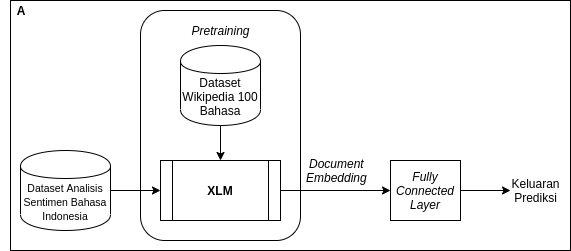
\includegraphics[width=1\textwidth]{resources/Arsitektur-TA-1.png}
		    \caption{ Ilustrasi \textit{finetuning} \textit{baseline} A.}
		    \label{fig:ilustrasi_solusi_1}
		\end{figure}

		\item \textbf{Tipe B}\\
		Pada tipe B ini, dilakukan ekperimen \textit{zero-shot learning}. Model XLM yang sudah dilatih pada data Wikipedia 100 bahasa hanya di-\textit{finetune} dengan data bahasa Inggris saja. Model ini kemudian langsung digunakan untuk melakukan klasifikasi sentimen bahasa Indonesia. Detail ilustrasi dapat dilihat pada Gambar \ref{fig:ilustrasi_solusi_2}.

		\begin{figure}[h]
		    \centering
		    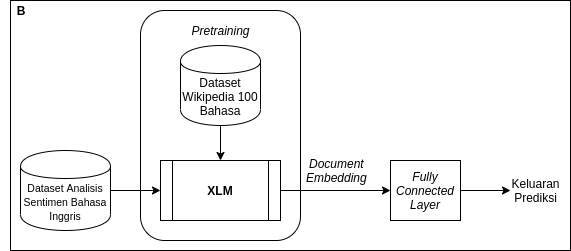
\includegraphics[width=1\textwidth]{resources/Arsitektur-TA-2.png}
		    \caption{ Ilustrasi \textit{finetuning} B.}
		    \label{fig:ilustrasi_solusi_2}
		\end{figure}

		\item \textbf{Tipe C}\\
		Pada tipe C ini, dilakukan ekperimen \textit{transfer learning} antar bahasa. Model XLM yang sudah dilatih pada data Wikipedia 100 bahasa di-\textit{finetune} dengan data bahasa Inggris. Model ini kemudian di-\textit{finetune} kembali dengan data bahasa Indonesia sebelum digunakan untuk melakukan klasifikasi sentimen bahasa Indonesia. Detail ilustrasi dapat dilihat pada Gambar \ref{fig:ilustrasi_solusi_3}.

		\begin{figure}[h]
		    \centering
		    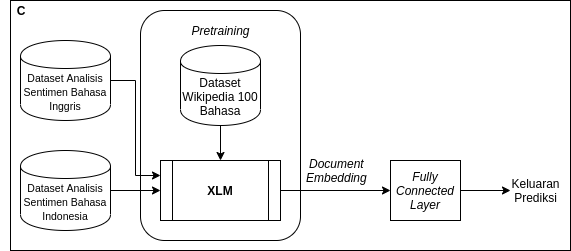
\includegraphics[width=1\textwidth]{resources/Arsitektur-TA-3.png}
		    \caption{ Ilustrasi \textit{finetuning} C.}
		    \label{fig:ilustrasi_solusi_3}
		\end{figure}
		
	\end{enumerate}

	Dalam setiap eksperimen, teks dipraproses terlebih dahulu menggunakan \textit{shared vocabulary} yang dibuat melalui \textit{Byte Pair Encoding (BPE)} hasil penelitian \parencite{LampleConneau2019}. Di setiap eksperimen juga akan digunakan \textit{callback} berupa \textit{EarlyStopping} dan \textit{ReduceLROnPlateau}. Penggunaan \textit{callback} \textit{EarlyStopping} digunakan agar model tidak \textit{overfit}. Sedangkan \textit{callback} \textit{ReduceLROnPlateau} digunakan untuk membantu model mencapai performa yang lebih baik.